%!TEX root = ../template.tex
%%%%%%%%%%%%%%%%%%%%%%%%%%%%%%%%%%%%%%%%%%%%%%%%%%%%%%%%%%%%%%%%%%%%
%% chapter5.tex
%% NOVA thesis document file
%%
%% Chapter with lots of dummy text
%%%%%%%%%%%%%%%%%%%%%%%%%%%%%%%%%%%%%%%%%%%%%%%%%%%%%%%%%%%%%%%%%%%%

\typeout{NT FILE chapter5.tex}%

\chapter{User Evaluation}
\label{cha:user_evaluation}
\setlength{\parskip}{0pt} 

This chapter introduces the user evaluation conducted in the scope of this dissertation. 
Section~\ref{sec:protocol} describes the methodology and procedures adopted for the evaluation, while Section~\ref{sec:results} presents the results obtained from the questionnaires, including a description of each type of questionnaire used and its intended purpose.

User testing was conducted in person with several groups of participants. \gls{VICARTE} experts, archaeologists (including the director of the Roman Ruins of Troia), and regular users provided more experienced and comprehensive feedback.
To differentiate and collect statistics from these groups independently, a question was added to the form to filter participants by professional specialty.
In this context, testing with experts was particularly relevant, considering these archaeologists had visited the site and examined the real objects. They contributed with their expertise in evaluating aspects such as the original glass texture generated REF and the tomb’s \gls{3D} model REF.

In total, 28 tests were carried out in presence: 16 with standard users, 3 with archaeologists, and 9 with \gls{VICARTE} members, including conservation and restoration specialists. The last group provided essential technical feedback in this field, as they were directly involved in interventions with the real objects.
The remaining users contributed a broader perspective on the usability of the \gls{VE}. Colleagues with prior \gls{VR} experience offered more informed insights, while standard users provided suggestions from a regular user’s perspective.

%In total were made twenty-eight tests, sixtheen texts with standart users, three tests with archaeologists, and with \gls{VICARTE} members, including conservation and restoration specialists, nine tests were conducted. %These allowed them to analyze and provide essential technical feedback in this field, people who made interventions in the real objects.

%Protocol/Questionnaires
\section{Protocol}
\label{sec:protocol}

This section describes the protocol adopted for the user evaluation questionnaire, which was organized into three subsections of the user form, each with a brief description and the corresponding test results.

The tests were fundamental in evaluating the usability 
%REF 
of the developed environment, as well as the sense of presence 
%REF 
and the overall experience. 
%REF.
The users had to answer a set of questions provided through Google Forms, divided into four sections. 

First, it was given a brief context of the project and the structure of the test.
Before using the headset, participants completed a personal questionnaire for statistical user analysis. 
Subsequently, it was time to make use of the \gls{HMD} and its right and left controllers.
The usage of the controllers and main buttons was explained. Then, the users were asked to complete a set of predefined tasks for the experience, which were:

\begin{enumerate}
\item{Try walking in continuous motion and/or teleporting in the environment.}
\item{Activate the 3D model of the funerary enclosure.}
\item{Walk to the tomb or select its blue icon to teleport.}
\item{Inside the tomb, point at an object until you see its blue outline and grab it.}
\item{Exit the tomb with the object in your hand.}
\item{With the object in your hand, use the other controller to move the slider and view its original appearance.}
\item{Release the object by releasing the side button on the controller.}
\item{Teleport to a Point of Interest by selecting one of the blue icons.}
\item{Activate the main menu and select the visible icon.}
\item{Close the main menu.}
\item{In the panel in front of you, select the Object ID 21684 and view the displayed information.}
\item{Walk to the blue panel and hover over the arrows to view object images after the intervention.}
\item{In the black panel in front of you, change the ground plane by selecting the "Toggle Layer" option and explore.}
\end{enumerate}

While the users were wearing the \gls{HMD} and controllers in their hands, as displayed in Figure \ref{fig:user}, the tasks were repeated to them, since the goal was not to evaluate memory, but usability.

During the tasks phase, time was measured for each user while interacting with the \gls{VR} environment, and using the headset. 
As shown in Table \ref{table:times}, the average time spent was around 10 minutes, with the exception of faster users and three cases where the application had to be restarted after users fell out of the environment, which increased the experience time.

\subsection{User Testing Setup}
\label{sec:setup}

The "Meta Horizon" app was employed to manage the headset. Through the app, with the "Cast" option activated, it was possible to view on the phone exactly what the user was viewing in real-time. 
With this feature, users were guided to perform the intended tasks and receive immediate assistance if any issues arose. 

After the initial setup with a USB connection, an \textbf{Android build} was generated in Unity, producing an \emph{.apk} file that allowed the application to run natively on the headset without requiring a cable. 
This provided greater flexibility during the evaluation. 
The \emph{Meta Quest Developer Hub} application was then used to transfer the \emph{.apk} file to the headset.

\begin{figure}[h!]
    \centering
    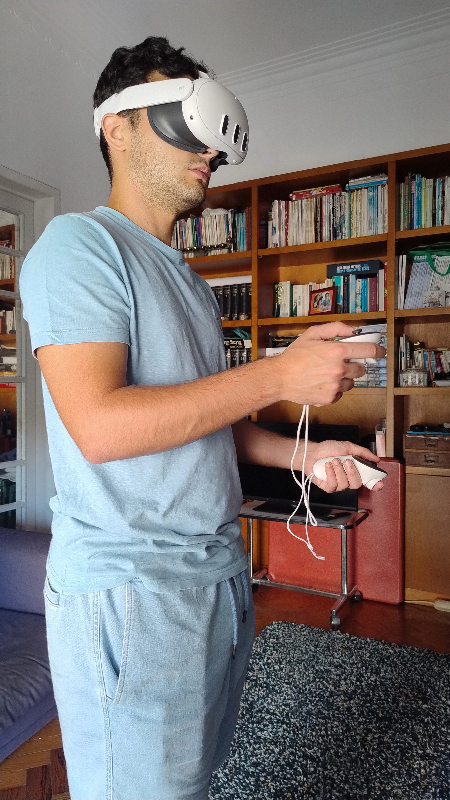
\includegraphics[width=0.35\linewidth]{test_user}
    \caption{User Testing the \gls{VR} Environment with the \gls{HMD} and controllers.} 
    \label{fig:user}
\end{figure}

\begin{table}[h!]
    \caption{Registered Times spent by each Participant to Execute the provided Tasks.} 
    \centering
    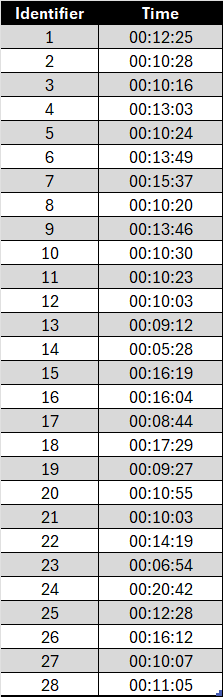
\includegraphics[width=0.25\linewidth]{Users/time_users}
    \label{table:times}
\end{table}

Finally, the users evaluated the experience through three separate sections. The first measured task success and the perception of key functionalities.
The following section evaluated the sense of presence in the environment. The third and final section assessed the overall experience within the environment.

\section{Tests Results}
\label{sec:results}

Starting with the subsection "User Analysis", which presents statistical information about the participants, followed by "Tasks Difficulty and Feedback", which reports their perceptions after completing the tasks.
In addition, the \gls{PQ} and \gls{UEQ} are employed to evaluate the overall experience and sensation. Finally, the subsection "Graphics Comparison" provides graphical representations that highlight relevant relationships between the users and their responses after performing the tasks.
\subsection{User Analysis}

This set of questions was designed to collect information on users' characteristics, enabling the identification of statistical differences and supporting the interpretation of the evaluation results. 
It includes demographic data such as age, gender, and education, along with information on professional or academic background.
In addition, it assesses prior experience with \gls{VR}, and digital technologies applied to \gls{CH}.
%video games, \gls{3D} environments,

\begin{figure}[h!]
    \centering
    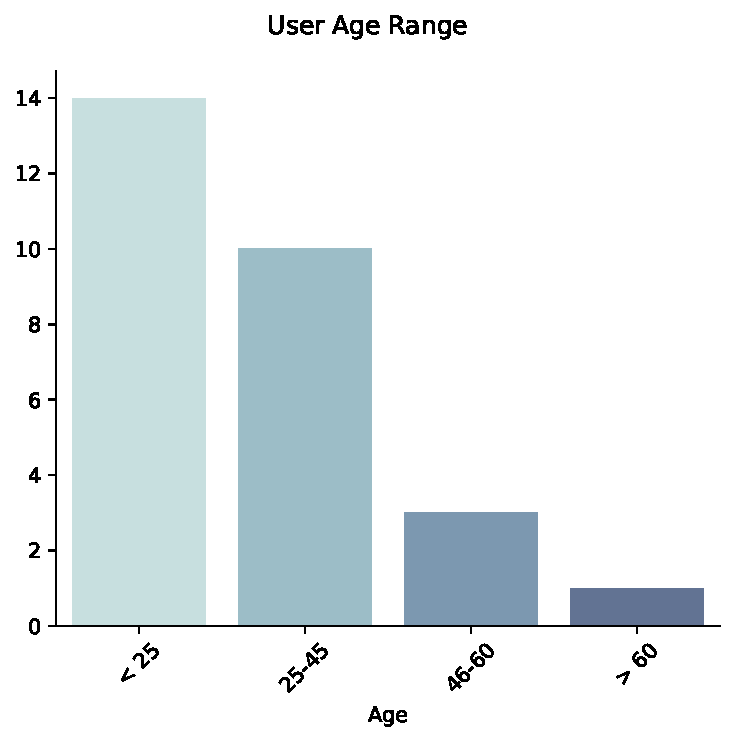
\includegraphics[width=0.5\linewidth]{Images/Age}
    \caption{Age Distribution of the Test Participants.} 
    \label{fig:age}
\end{figure}

The bar plot in Figure \ref{fig:age} illustrates the distribution of participants across age groups. A decreasing trend of users can be observed with increasing age. Notably, the majority of participants, 86\%, are younger than 45 years old.
%As shown in Table X, and as expected, users specialists in conservation and restoration, or archaeology are predominantly represented in the age groups above 25 years.
We can conclude that we have a good age range despite a smaller sample of older people.

\begin{figure}[h!]
    \centering
    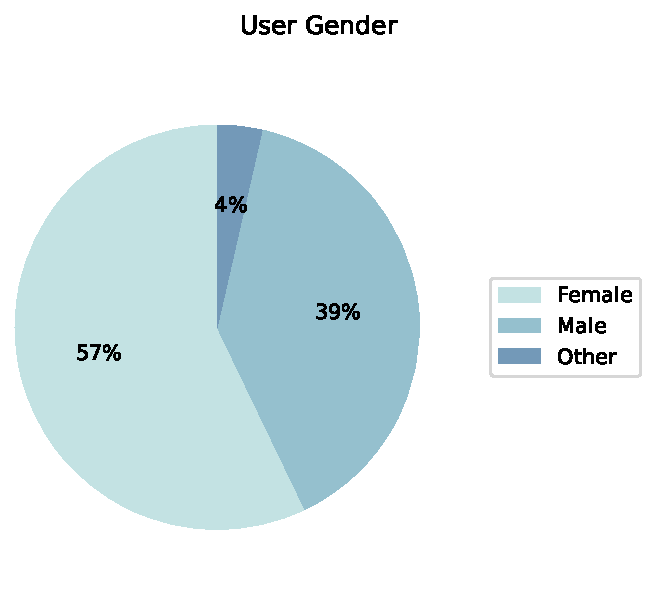
\includegraphics[width=0.4\linewidth]{Images/Gender}
    \caption{Gender Distribution of the Test Participants.} 
    \label{fig:gender}
\end{figure}

There is a diversified gender distribution as we can see in Figure \ref{fig:gender}.

\begin{figure}[h!]
    \centering
    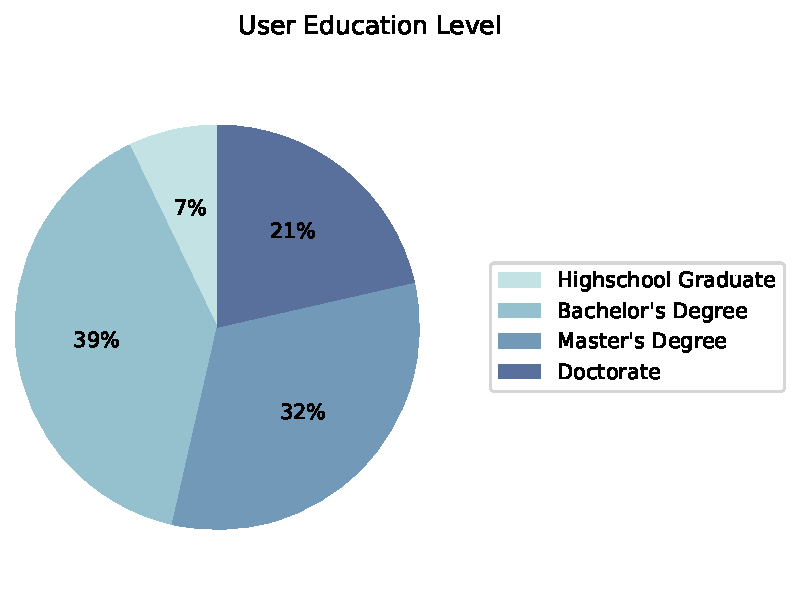
\includegraphics[width=0.5\linewidth]{Images/Education}
    \caption{Education Level Distribution of the Test Participants.} 
    \label{fig:education}
\end{figure}

In the pie chart of Figure \ref{fig:education}, the educational degrees of the participants is depicted. 
The distribution indicates a predominance of higher education (bachelor, master, and doctorate degees), whereas only a small proportion of participants reported lower levels of education.


\begin{figure}[h!]
    \centering
    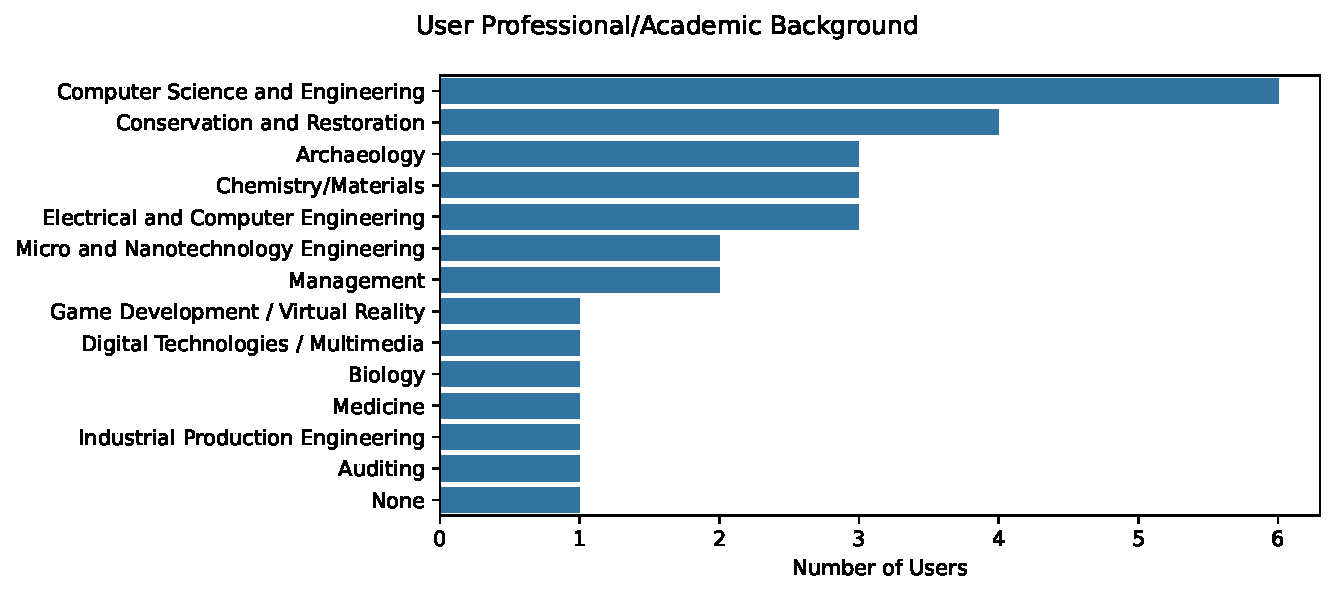
\includegraphics[width=1\linewidth]{Images/Backroumd}
    \caption{Distribution of Training Levels among Participants.} 
    \label{fig:background}
\end{figure}

In Figure \ref{fig:background}, a horizontal bar plot illustrates the distribution of participants’ technical backgrounds. 
The areas are ordered in descending frequency, with priority given to those most relevant for this thesis. 
This results in a meaningful sample, comprising mainly technology developers, specialists in conservation and restoration, and archaeologists working in contexts comparable to the site under study.

\begin{figure}[h!]
    \centering
    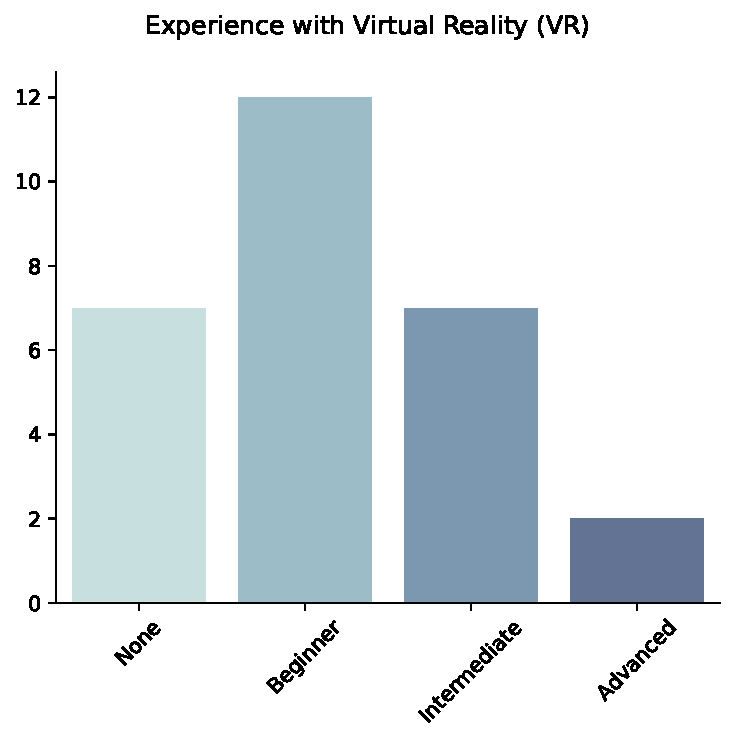
\includegraphics[width=0.55\linewidth]{Images/VR_experience}
    \caption{\gls{VR} Experience Levels among Participants.} 
    \label{fig:VR_experience}
\end{figure}

As illustrated in Figure \ref{fig:VR_experience}, it is evident that the majority of the participants have prior experience with \gls{VR}, while only a small portion are experts.

\begin{figure}[h!]
  \centering
  \begin{subfigure}[b]{0.47\textwidth}
      \centering
      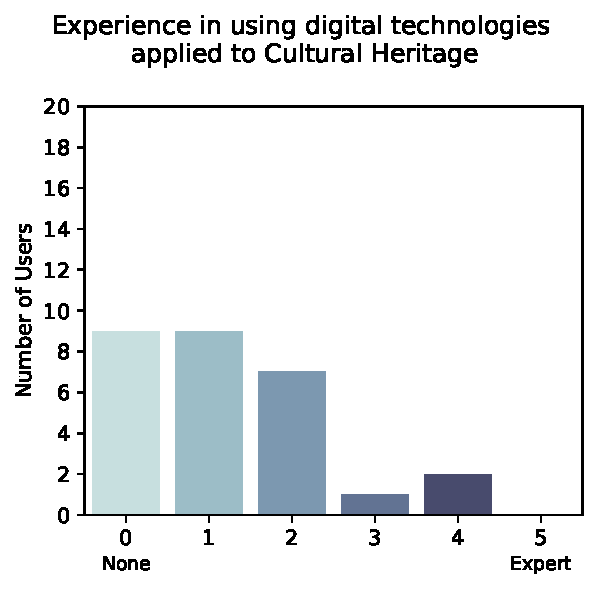
\includegraphics[width=1.0\textwidth]{Images/Using2}
      %\caption{Experience in using technologies.}
      \label{fig:Using}
  \end{subfigure}
  \hfill
  \begin{subfigure}[b]{0.47\textwidth}
      \centering
      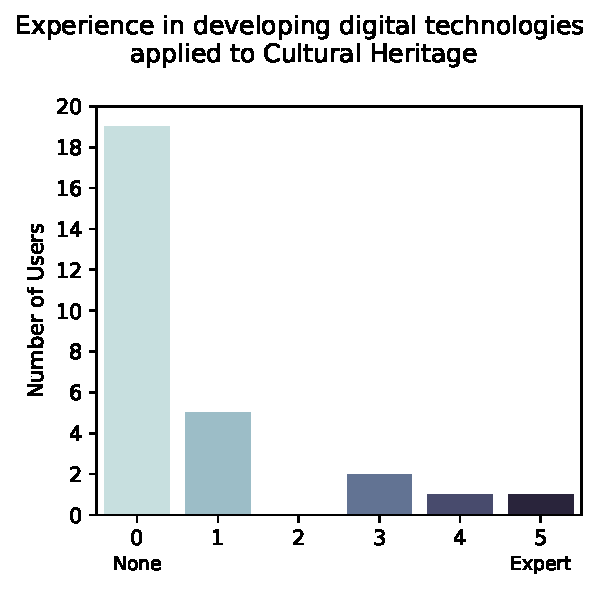
\includegraphics[width=1.0\textwidth]{Images/Developing2}
      %\caption{Experience in developing technologies.}
      \label{fig:Developing}
  \end{subfigure}
     \caption{Participants’ Experience with Digital Technologies Applied to \gls{CH}.}
     \label{fig:hertiage_techs}
\end{figure}
\FloatBarrier

%From the two represented distributions represented in Figure \ref{fig:hertiage_techs} of using and developing techologies related to heritage, that they have opposite results. The majority of the participants have used these tecnologies, while only a small quantity has developed.
%In this case, the most important thing for evaluation is the use, which will be who will actually use the developed system, while the developers are useful to give more technical feedback, or suggestions for improvements in terms of efficiency, for example.
The two distributions in Figure \ref{fig:hertiage_techs} show a clear disparity between participants' experiences in using and developing digital heritage technologies. Most participants (19) report having some experience as users, generally clustering around moderate levels (ratings 1–2). 
In contrast, almost all participants (18) report no development experience.
For evaluation purposes, the key factor is the intended use of the system, as this determines who will actually engage with it. Developers remain valuable mainly for offering technical feedback and suggestions for improvements, such as efficiency.


% \begin{figure}[h!]
%     \centering
%     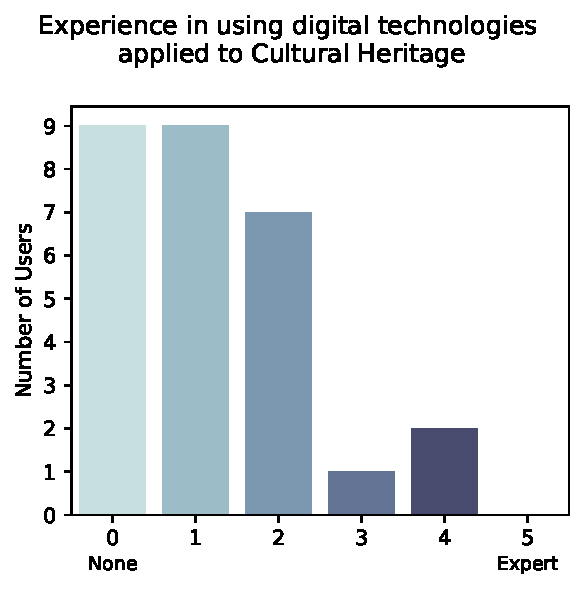
\includegraphics[width=0.6\linewidth]{Images/Using}
%     \caption{\gls{VR} Experience distribution of the test participants.} 
%     \label{fig:using}
% \end{figure}


% \begin{figure}[h!]
%     \centering
%     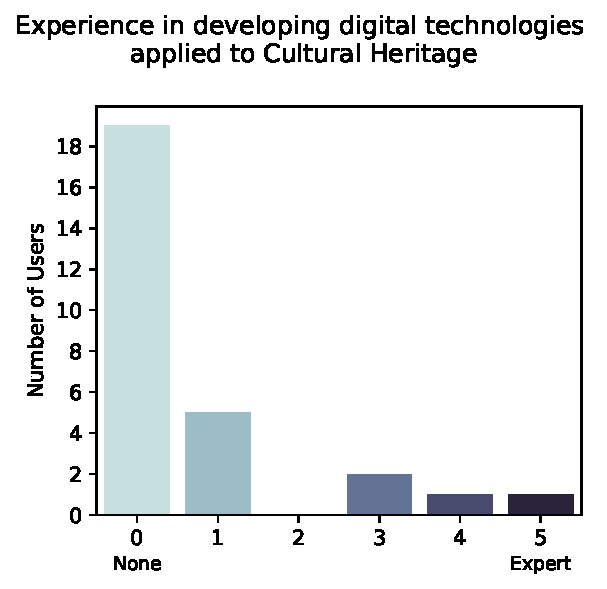
\includegraphics[width=0.6\linewidth]{Images/Developing}
%     \caption{\gls{VR} Experience distribution of the test participants.} 
%     \label{fig:developing}
% \end{figure}



\subsection{Tasks Difficulty and Feedback}

This segment of questions was answered immediately after the users completed their tasks in the \gls{VE}.
The first question in this section used a 5-point Likert scale to measure the perceived difficulty of each task, providing insights that may support future improvements or adjustments to the \gls{UI}.
The second and final question in this section presented a list of ten statements, tailored to the evaluation of this environment, which users rated on a 5-point Likert scale according to their level of agreement.
This helps to capture more specific perceptions regarding each relevant functionality and the overall experience within the environment.
%\subsection{General Feedback}

\begin{figure}[h!]
    \centering
    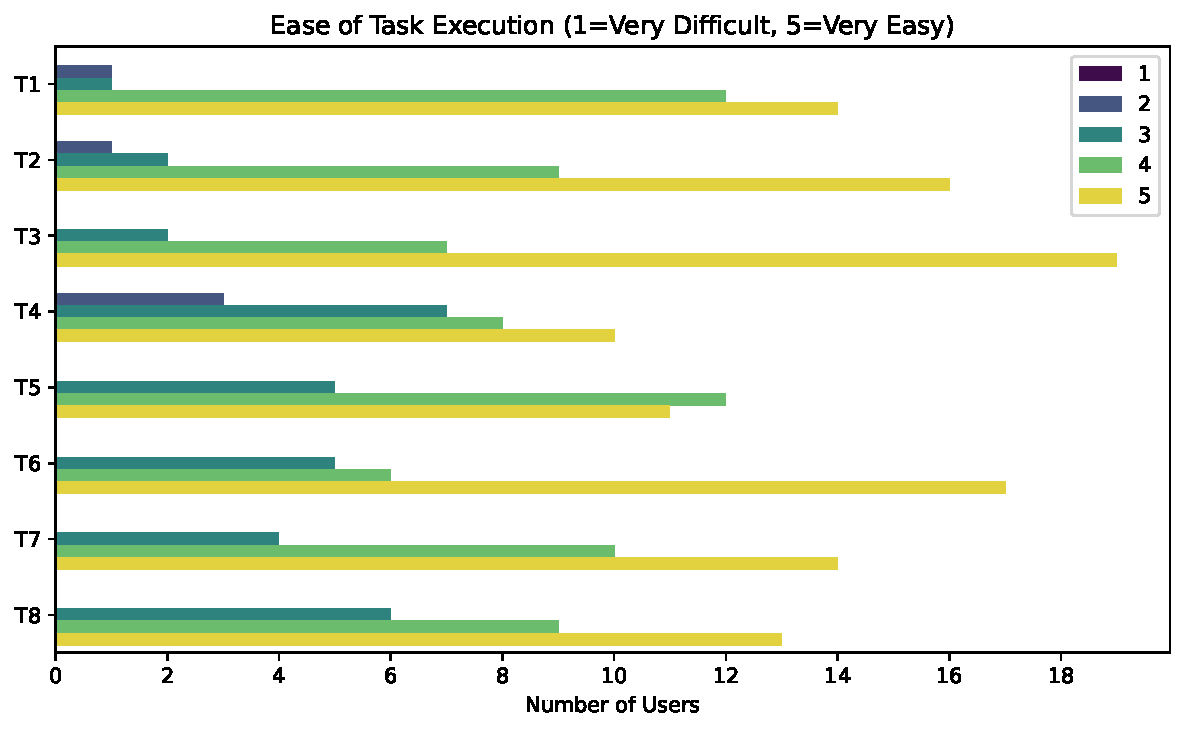
\includegraphics[width=0.8\linewidth]{Images/Task_Difficulty}
    \caption{Perceived Task Ease among Participants.} 
    \label{fig:diffculty}
\end{figure}

Analyzing the graph in Figure \ref{fig:diffculty}, we can observe the overall ease of completing the tasks.
The results indicate that the most difficult task was T4 – "Access to the main menu", likely because participants did not remember that it required pressing the back button on the right controller. 
Task T5 – "View original appearance of the object with the slider", also presented difficulty, possibly due to the diffculty of interacting with the slider bar. 
It is important to note that this issue was later improved by making the entire slider bar visible and removing the need sometimes to cross the arms to move it. 
This improvement is further explained in Section \ref{sec:improvements}.

% The results demonstrate
% It IS POSSIBLE TO OBSERVE
%tHE RESULTS INDICATE
%tHE VALUES DENOTE
%SHOWS

\begin{figure}[h!]
    \centering
    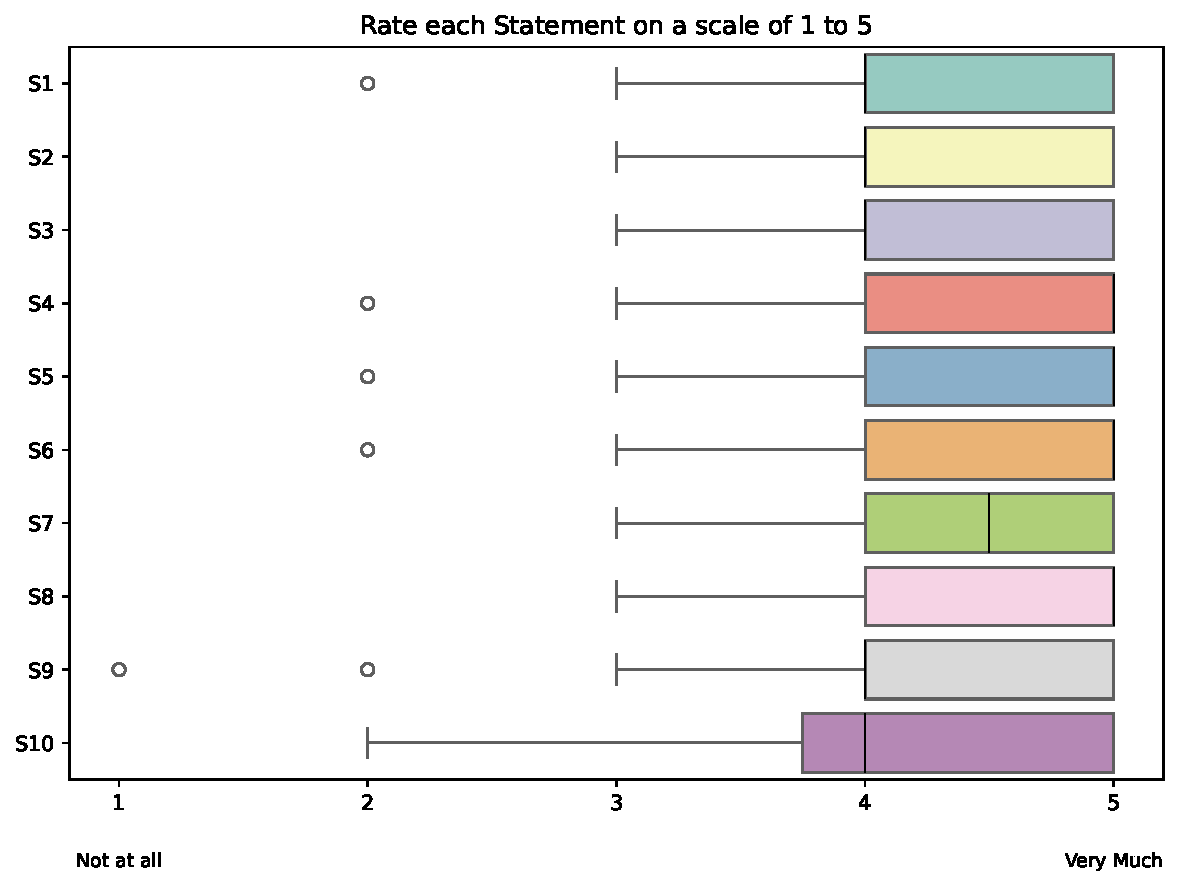
\includegraphics[width=0.8\linewidth]{Images/Task_Overview_}
    \caption{Participants’ Agreement with Task-Related Statements.} 
    \label{fig:overview}
\end{figure}
\FloatBarrier


The results shown in Figure \ref{fig:overview} indicate a general agreement among users with the statements concerning their interaction, exploration, and navigation within the environment.
In particular, statements 4, 5, and 6 received the highest levels of agreement, regarding the effectiveness of the slider in displaying transformations and the engagement of the information provided about the objects.
The median values of all statements range between 4 and 5, highlighting a very positive outcome.
%highlighting ou which

\subsection{Presence Questionnaire (PQ)}

The evaluation of presence was conducted using the Portuguese validated version of the Presence Questionnaire, adapted by Vasconcelos-Raposo et al. \cite{Vasconcelos-Raposo03102021} was used, from which eleven items were removed 
"in order to improve the validity of the constructs and their internal consistency."
The original Presence Questionnaire by Witmer et al. \cite{10.1162/105474698565686} consists of thirty-two questions, covering four major factor categories: Control, Sensory, Distraction, and Realism.
In the translated version, ten of the twenty-one validated and translated questions were selected, as they were considered the most relevant for this research. 
Questions addressing less important topics, such as sounds during the experience, were excluded. This questionnaire section was applied using a 5-point Likert scale.

\begin{figure}[h!]
    \centering
    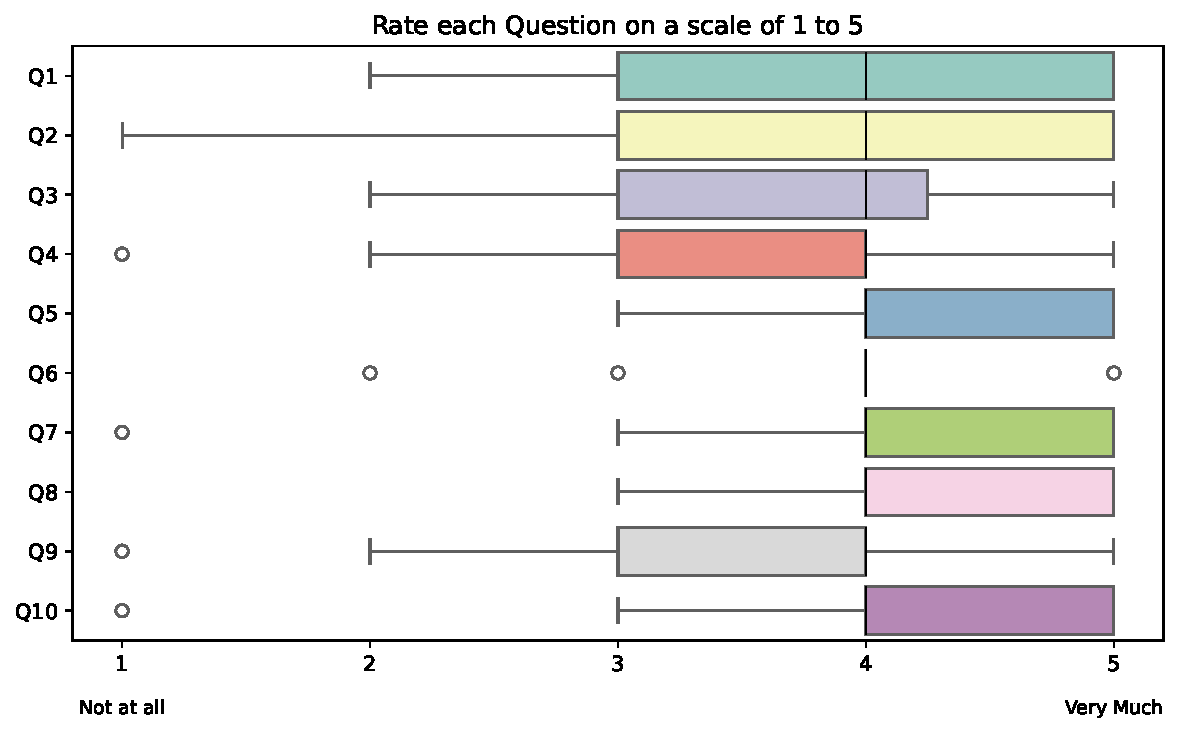
\includegraphics[width=0.9\linewidth]{Images/PQ}
    \caption{Perceived Sense of Presence among Participants.} 
    \label{fig:PQ}
\end{figure}

It is represented in Figure \ref{fig:PQ} the participants’ sense of presence during this evaluation.%experience.

It is interesting to note that Q6 – "How proficient in moving and interacting with the virtual environment did you feel at the end of the experience?" – shows that quartiles 1, 2, and 3 coincide at the value 4. 
This indicates a very strong consensus among participants, with at least 50\% reporting good navigation and understanding of the environment after the experience, reflected in a median score of 4 out of 5. 
Overall, most participants rated their proficiency as 4, showing strong agreement, with only a few outliers providing lower or higher ratings.
%adiciono questoes 5 e 8 que comprovam  sentimento de imersividade, sem outliers
\subsection{User Experience Questionnaire (UEQ-S)}

The overall user experience was measured using the Portuguese version of the User Experience Questionnaire\footnote{\url{https://www.ueq-online.org/}}, constructed by Laugwitz et al. \cite{inproceedings}, and translated by Cota et al. \cite{article_t}.

The UEQ-S is the short version of the User Experience Questionnaire (UEQ), comprising a list of eight items selected from the original twenty-six. \cite{article_ueq}. These items are grouped into two meta-dimensions, illustrated in Figure \ref{fig:scale}: pragmatic quality and hedonic quality, each containing four items.
In addition, the mean value across all items is reported as an overall \gls{UX} score.
The questionnaire is structured around pairs of contrasting attributes that may describe the system. Participants provide their evaluation on a seven-point scale, where each circle represents a gradation between the two opposites.
%is based on

%These pairs address five factors: Attractiveness, Perspicuity, Dependability, Efficiency, Novelty, and Stimulation.  

\begin{figure}[h!]
    \centering
    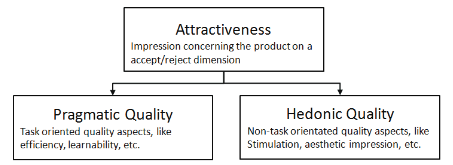
\includegraphics[width=0.9\linewidth]{Images/scale}
    \caption{Grouping of the two quality attributes \cite{article_sca}.} 
    \label{fig:scale}
\end{figure}


\begin{figure}[h!]
    \centering
    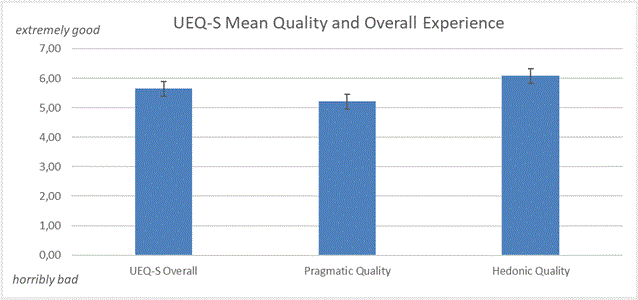
\includegraphics[width=0.9\linewidth]{Images/UEQ3}
    \caption{Overview of the \gls{UEQ} Evaluation Distribution among Test Participants.} 
    \label{fig:UEQ2}
\end{figure}


The \gls{UEQ} results, as demonstrated in Figure \ref{fig:UEQ2}, show a highly positive overall experience. 
The evaluation factor hedonic quality, reflecting user satisfaction and enjoyment, was particularly high, while pragmatic quality denoted the system’s usefulness and effectiveness.
\begin{figure}[h!]
    \centering
    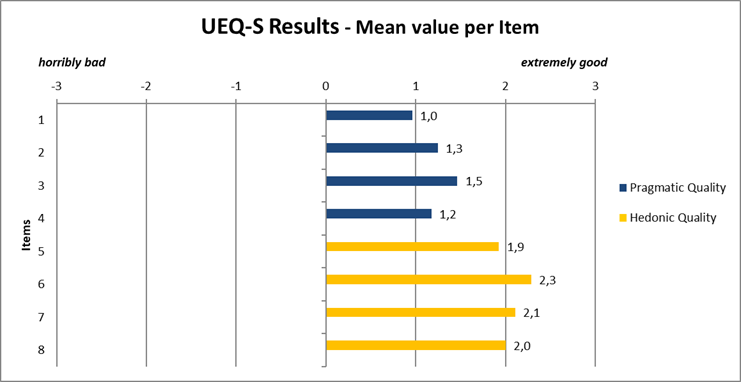
\includegraphics[width=0.9\linewidth]{Images/UEQ}
    \caption{Mean value of \gls{UEQ} Items of the Participants' Experience.} 
    \label{fig:UEQ1}
\end{figure}
\begin{table}[h!]
    \caption{\gls{UEQ} Items, their Mean responses, Standard Deviations, and the corresponding Opposite Pairs by Scale.}
    \centering
    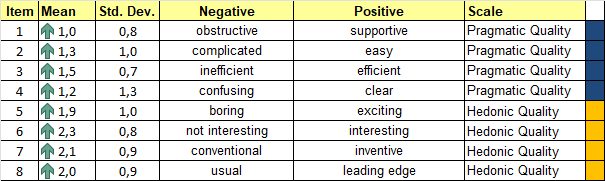
\includegraphics[width=0.9\linewidth]{Images/table_ueq}
    \label{table:table_UEQ}
\end{table}


On a scale from -3 to 3, Figure \ref{fig:UEQ1} illustrates the mean responses of the participants per item.  
We can conclude that there is a good average, especially in the Hedonic Quality.  
The y-axis shows the list of \gls{UEQ} items, with participants grouped by scale dimension: Pragmatic or Hedonic Quality.  
Table \ref{table:table_UEQ} supports this graphic with this and more relevant information of the \gls{UEQ} used.
\FloatBarrier

\subsection{Graphics Comparison}
\label{sec:comparison}

\begin{figure}[h!]
    \centering
    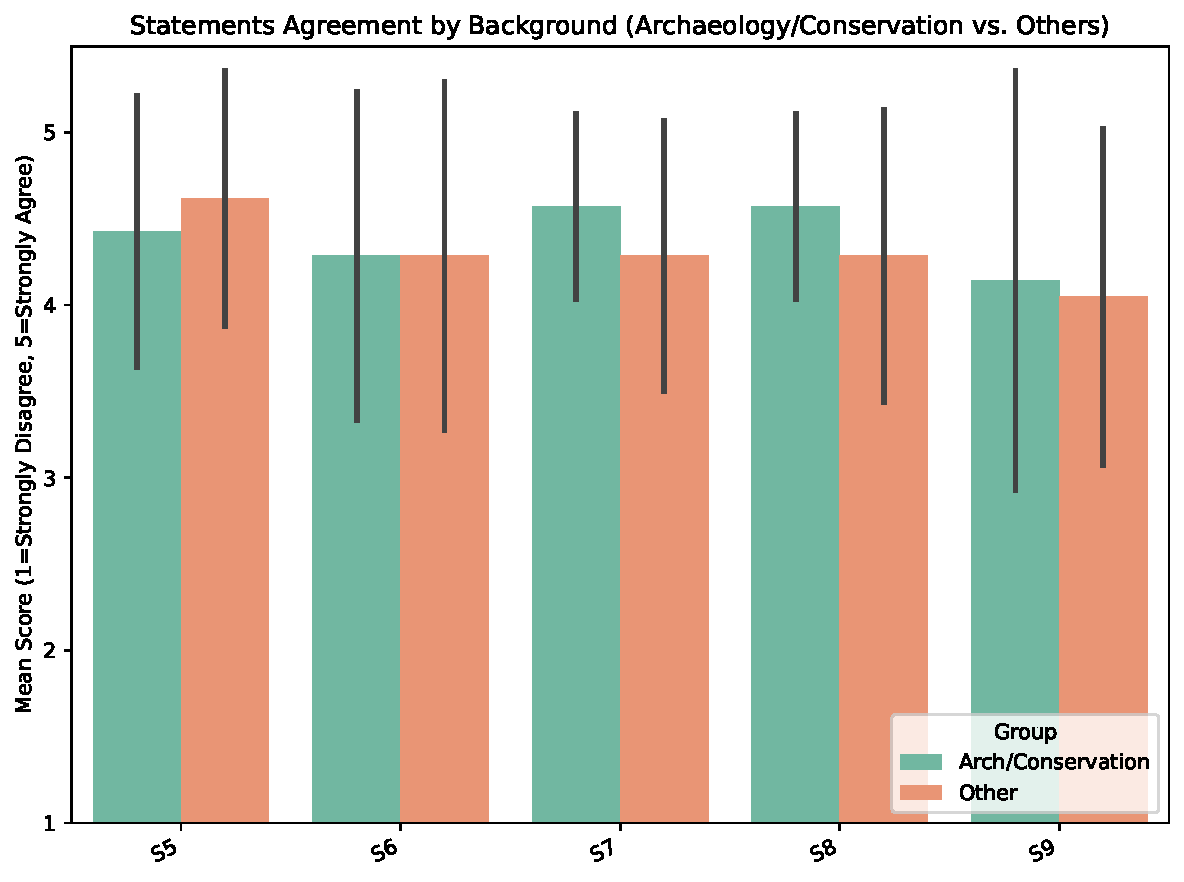
\includegraphics[width=0.8\linewidth]{Images/statements_by_group2}
    \caption{Comparison between Participant Groups, regarding Agreement with Statements about their Experience.} 
    \label{fig:statements_background}
\end{figure}

The graph illustrated in Figure \ref{fig:statements_background} compares agreement with statements, distinguishing participants with a background in Archaeology/Conservation from those in other fields. The error bars represent the standard deviation, indicating the variability in the responses.
The statements correspond to the ones used on the y-axis of Figure \ref{fig:overview}, with a focus on those considered most meaningful for an Archaeology or Conservation/Restoration specialization.
Those are: 

\begin{itemize}
  \item S5 - I clearly distinguish between the artifact's original and restored state.
  \item S6 - The information provided helped me better understand the artifact.
  \item S7 - The experience contributed to a better understanding of the site.
  \item S8 - The experience helped me better understand the presented artifacts.
  \item S9 - The experience provoked a sense of presence in the historical site.
\end{itemize}

In general, as represented above, specialists provided a better average score to the statements, except statement 5, presumably due to the greater critical demand of professionals who have direct experience with artifacts in the field of conservation and restoration.

\begin{figure}[h!]
     \centering
     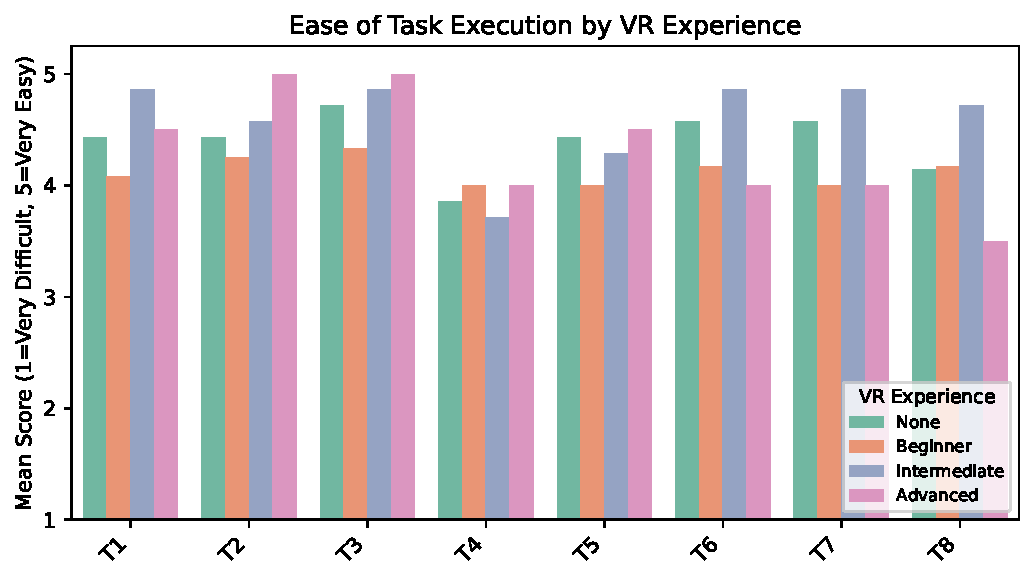
\includegraphics[width=0.8\linewidth]{Images/tasks_byVR_experience}
     \caption{Ease of Task Execution according to Participants’ \gls{VR} Experience.} 
     \label{fig:tasks_byVR_experience}
 \end{figure}

The results presented in Figure \ref{fig:tasks_byVR_experience} indicate a general ease in completing the tasks among participants with higher levels of experience in \gls{VR}. 
However, in some cases, the scores for the Intermediate group exceeded those of the Advanced group (specifically in T1, T6, T7, and T8). 
This outcome may be explained by the fact that, as illustrated in Figure \ref{fig:VR_experience}, only two participants were classified as "Advanced", representing a very small sample that may not provide fully reliable results.

\begin{figure}[h!]
    \centering
    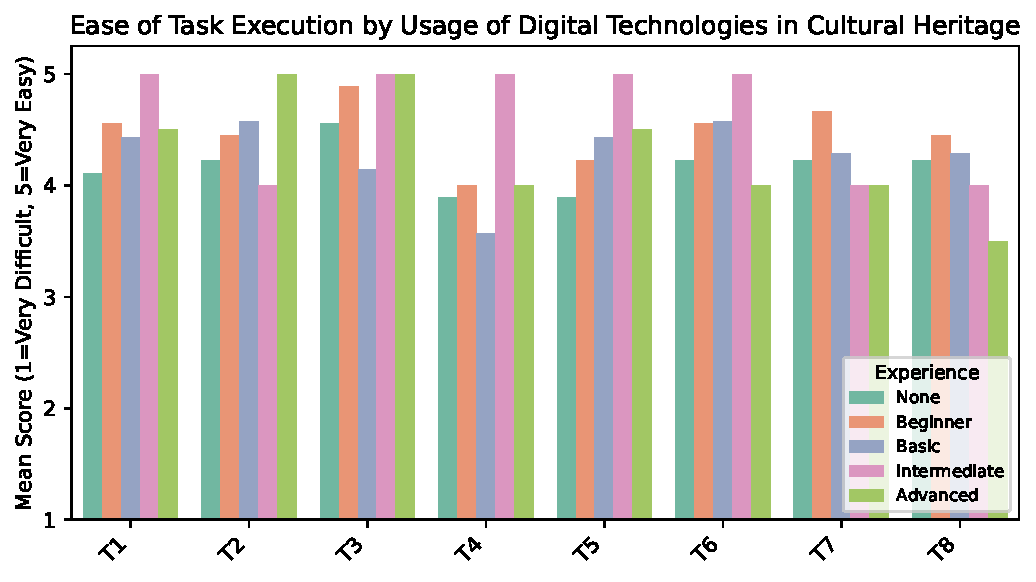
\includegraphics[width=0.8\linewidth]{Images/tasks_byheritage_experience}
    \caption{Ease of Task Execution according to Participants’ Experience with Technologies applied to \gls{CH}.} 
    \label{fig:tasks_byheritage_experience}
\end{figure}

The bar chart in Figure \ref{fig:tasks_byheritage_experience} demonstrates that users with greater experience in technologies applied to \gls{CH} generally found the tasks easier to execute, except for T7 – "Access a point of interest", and T8 – "Change the base (ground) plan".

\begin{figure}[h!]
    \centering
    \includegraphics[width=0.8\linewidth]{Images/presence_byVR_experience}
    \caption{Participants’ reported Sense of Presence according to their \gls{VR} Experience.} 
    \label{fig:presence_byVR_experience}
\end{figure}


In Figure \ref{fig:presence_byVR_experience}, a bar graph illustrates the Sense of Presence results from the \gls{PQ}, organized by participants’ \gls{VR} experience. 
Remarkably, users with no previous \gls{VR} experience reported, in various questions (Q2, Q3, Q5, and Q8), a stronger sense of presence than those proficient.

\FloatBarrier
\section{Discussion}
\label{sec:eval_discussion}

Overall, the results obtained of the User Analysis were balanced, showing a generally younger age group with higher education levels. Professional backgrounds were well distributed, with a larger proportion in Computer Science and Engineering, and Conservation and Restoration.
Most participants had at least some prior experience with \gls{VR} and in using digital technologies applied to \gls{CH}. The tasks were generally completed with ease, as showed in Figure \ref{fig:diffculty}. In addition, the \gls{PQ} results indicated a good median sense of presence among participants, and the \gls{UEQ} reflected a very positive overall user experience as demonstrated by the mean.
In Section \ref{sec:comparison}, participants with specialist knowledge in Conservation and Restoration, and Archaeology showed slightly higher average scores on statements related to their field, compared to others. As expected, prior experience with \gls{VR} and in technologies associated with \gls{CH} helped participants solve the tasks.
Finally, the sense of presence was generally stronger when participants were previously engaged with \gls{VR}, although there were some exceptions for certain \gls{PQ} items.

\subsection{Improvements After User Testing}
\label{sec:improvements}

Some minor improvements were made following user testing. These mainly concerned the \gls{UI} and small implementation bugs:

\begin{itemize}
 \item Enabled the possibility to activate or deactivate the model throughout the entire experience, rather than only the first time. Previously, the collider component that allowed this functionality was deactivated after the user entered the tomb.
 \item Allowed teleportation to the tomb icon even when the menu panel was open. Those were interfering, so previously, the teleportation was only possible when the panel was closed.
 \item Added a legend when selecting the correct option in the main menu to guide users.
 \item Simplified slider interaction: it is no longer necessary to cross the arms to move the slider. When grabbing the object with the right controller, the bar now correctly repositions on the corresponding side.
 \item Original Glass Texture Improvements: Adjusted parameters for object ID 2676. Enhanced the realism of the texture by adding a slight blue tint, as experts indicated that these Roman glasses tended to have a bluish hue.
 \item Tomb Interaction: Improved the definition of the tomb limits, increasing the coordinate precision on both sides.
\end{itemize}

